% preamble.tex

\usepackage{lmodern}

\usepackage{xeCJK}
\usetheme{CambridgeUS} % try Madrid, Pittsburgh
\usecolortheme{beaver}
\usefonttheme[]{serif} % try "professionalfonts"

\setbeamertemplate{itemize items}[default]
\setbeamertemplate{enumerate items}[default]

\usepackage{amsmath, amsfonts, latexsym, mathtools}
% \usepackage{fdsymbol} % for poker
\newcommand{\set}[1]{\{#1\}}
\DeclareMathOperator*{\argmin}{\arg\!\min}

\definecolor{bgcolor}{rgb}{0.95,0.95,0.92}

% colors
\newcommand{\red}[1]{\textcolor{red}{#1}}
\newcommand{\redoverlay}[2]{\textcolor<#2>{red}{#1}}
\newcommand{\green}[1]{\textcolor{green}{#1}}
\newcommand{\blue}[1]{\textcolor{blue}{#1}}
\newcommand{\blueoverlay}[2]{\textcolor<#2>{blue}{#1}}
\newcommand{\teal}[1]{\textcolor{teal}{#1}}
\newcommand{\purple}[1]{\textcolor{purple}{#1}}

% colorded box
\newcommand{\rbox}[1]{\red{\boxed{#1}}}
\newcommand{\gbox}[1]{\green{\boxed{#1}}}
\newcommand{\bbox}[1]{\blue{\boxed{#1}}}
\newcommand{\pbox}[1]{\purple{\boxed{#1}}}

\usepackage{pifont}
\usepackage{wasysym}

\newcommand{\cmark}{\green{\ding{51}}}
\newcommand{\xmark}{\red{\ding{55}}}
%%%%%%%%%%%%%%%%%%%%%%%%%%%%%%%%%%%%%%%%%%%%%%%%%%%%%%%%%%%%%%
% for fig without caption: #1: width/size; #2: fig file
\newcommand{\fig}[2]{
  \begin{figure}[htp]
    \centering
      \includegraphics[#1]{#2}
  \end{figure}
}

\usepackage{tikz}
\usetikzlibrary{positioning}
\usepackage{adjustbox}
% \resizebox{0.90\textwidth}{!}{% chain-intersection.tex

\begin{tikzpicture}[node distance = 0.00cm]
  \node (abcd) [] {
\includegraphics[scale = 0.30]{figs/chain-abcd}};
  \uncover<2->{\node (cap1) [red, right = of abcd] {$\cap$};}
  \node (acbd) [right = of cap1] {
\includegraphics[scale = 0.30]{figs/chain-acbd}};
  \uncover<2->{\node (cap2) [red, right = of acbd] {$\cap$};}
  \node (acdb) [right = of cap2] {
\includegraphics[scale = 0.30]{figs/chain-acdb}};

  \node (eq) [purple, right = of acdb] {$=$};
  \node (poset-abcd-hasse-1) [right = of eq] {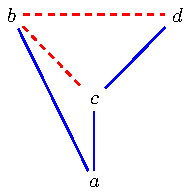
\includegraphics[scale = 0.40]{figs/poset-abcd-hasse-1}};
\end{tikzpicture}
}

\newcommand{\titletext}{1-13 Boolean Algebra}
\newcommand{\ps}[1]{\mathcal{P}(#1)}
\newcommand{\N}{\mathbb{N}}
\newcommand{\R}{\mathbb{R}}
\newcommand{\CP}{\mathbb{C}}

\newcommand{\thankyou}{
  \begin{frame}[noframenumbering]{}
    \fig{width = 0.50\textwidth}{figs/thankyou.png}
  \end{frame}
}
